\begin{figure}[ht]
	\centering
	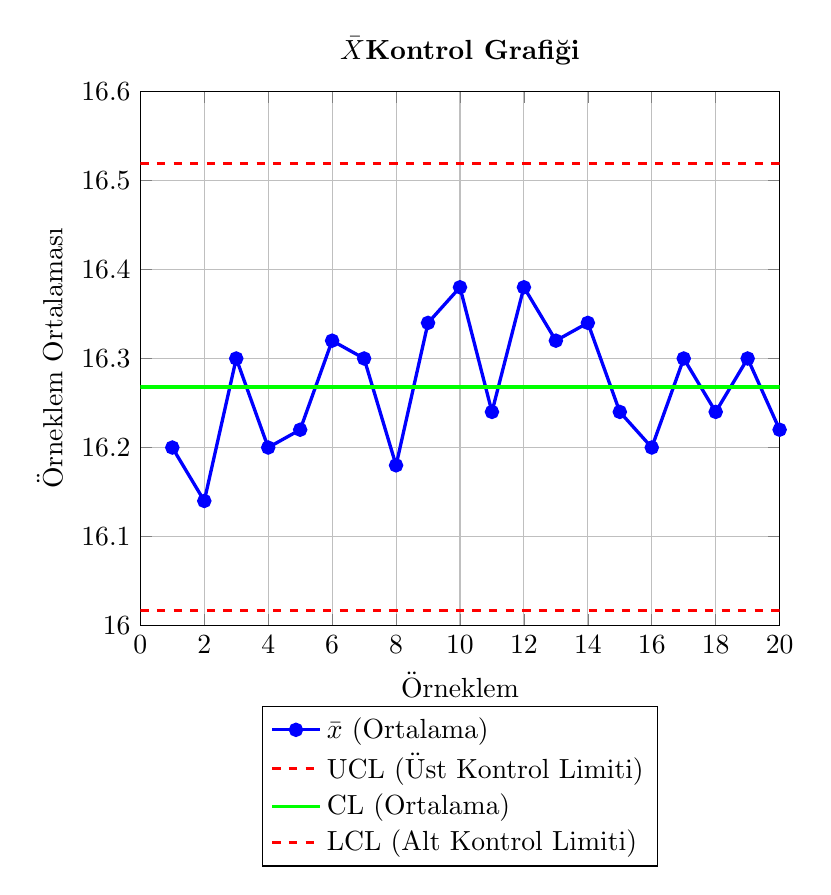
\begin{tikzpicture}
		\begin{axis}[
			title={\bfseries $\bar{X}$Kontrol Grafiği},
			xlabel={Örneklem},
			ylabel={Örneklem Ortalaması},
			xmin=0, xmax=20,
			ymin=16, ymax=16.6,
			grid=both,
			    legend style={at={(0.5,-0.15)}, anchor=north},
			    legend cell align=left,
			    legend entries={},
			width=0.8\textwidth,
			]

			\addplot[
			color=blue,
			mark=*,
			very thick
			] coordinates {
				(1, 16.2) (2, 16.14) (3, 16.3) (4, 16.2) (5, 16.22) 
				(6, 16.32) (7, 16.3) (8, 16.18) (9, 16.34) (10, 16.38)
				(11, 16.24) (12, 16.38) (13, 16.32) (14, 16.34) (15, 16.24) 
				(16, 16.2) (17, 16.3) (18, 16.24) (19, 16.3) (20, 16.22)
			};
			\addlegendentry{$\bar{x}$ (Ortalama)}
			
			% UCL çizgisi
			\addplot[
			color=red,
			dashed,
			very thick
			] coordinates {
				(0, 16.5188) (20, 16.5188)
			};
			\addlegendentry{UCL (Üst Kontrol Limiti)}
			
			% CL çizgisi
			\addplot[
			color=green,
			very thick
			] coordinates {
				(0, 16.2680) (20, 16.2680)
			};
			\addlegendentry{CL (Ortalama)}
			
			% LCL çizgisi
			\addplot[
			color=red,
			dashed,
			very thick
			] coordinates {
				(0, 16.0172) (20, 16.0172)
			};
			\addlegendentry{LCL (Alt Kontrol Limiti)}
			
		\end{axis}
	\end{tikzpicture}
	\caption*{}
\end{figure}


ilk dikkat çeken pattern, ortalama etrafında salınım yapan gözlemlerdir. Evet, istatistiksel olarak bu sürecin “yeterli” olduğunu söyleyebiliriz. Sebebini ise “kontrol limitlerine ulaşan herhangi bir gözlem (phase 2) gerçekleşmemiş” olarak açıklayabiliriz. Grafiğin yaptığı salınım, özellikle birbiri ardına olan gözlemlerdeki ortalama farklılıkları, süreci inceleyen bizlere şu noktaların düşünülmesi gerektiği hakkında bazı fikirler verir: 

\begin{enumerate}[label=\Roman{enumi}.]
	\item 
	Örneğimizdeki süreçte ağırlığı takip edilen dry bleach’ı işleten ve ambalajlayan makinelerin kalibrasyonunda bir sıkıntı oluyor veya fabrikanın üretim bandında prosedür dışı beklenmeyen bir olay gerçekleşiyor olabilir. 
	\item 
	Eğer makineler bir operatör yardımı ile çalıştırılıyor ise, birbirinden farklı çalışma stillerine sahip olan çalışanların yarattığı bir sorun olabilir. Çalışan ve gözlemler arasında bir bağlantı var mı diye bakılmalıdır. 
	\item 
	Süreç sürekli incelendiği için yapılan denemeler belki de birbirini etkiliyor, üretim hattı düzgün koşullar ile incelenmiyor veya yapılan gözlemler birbirinden farklı makineler, departmanlar veya koşullar arasında yapıldığından deney aynı çıktıları sağlayamıyor olabilir. \\
	
	Xbar Kontrol Kart'ı ve süreç hakkındaki yorumlamalardan sonra artık S Kontrol Kartı’nın kontrol limitlerini hesaplamaya, grafiğini çizmeye ve ardından (a) şıkkı için nasıl yorumlanması gerektiği hakkında konuşulacaktır. 
	
\end{enumerate}
